\OnehalfSpacing
% ---
\chapter{Introdução}
% ---

O artigo \cite{Wang2013} ...

A Figura \ref{fig:smart_meter} ilustra ...


\begin{figure}[ht]
\begin{center}
    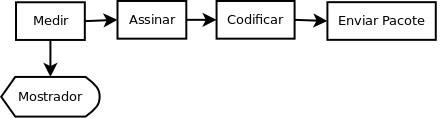
\includegraphics[width=0.5\textwidth]{figs/smartmeter.png}
\end{center}
\caption{Titulo da Figura}
\label{fig:smart_meter}
\end{figure}

% --------------------------------------------------------
\section{Objetivos}
% --------------------------------------------------------

Seus objetivos...

A Tabela \ref{tab:table1} mostra ...


\begin{table}[ht]
\centering
\caption{Titulo da Tabela}
\label{tab:table1}
\begin{tabular}{|l|l|l|}
\hline
\textbf{Item 1} & \textbf{Item 2} & \textbf{Item 3} \\ \hline
A         & D       & G        \\ \hline
B         & E       & H        \\ \hline
C         & F       & I       \\ \hline
\end{tabular}
\end{table}

\subsection{Subseção}

\lipsum[3-56]

\subsubsection{Subsubseção}

\lipsum[3-56]

\subsubsubsection{Subsubsubseção}

\lipsum[3-56]

%Essa dissertação tem como objetivo principal propor uma aplicação para aquisição e autenticação dos dados de consumo gerados por SMs usando uma nuvem computacional.

%Com objetivos secundários:

%\begin{itemize}
%	\item Verificar a pertinência do uso da arquitetura SGX de forma a satisfazer os requisitos de segurança da informação;

%	\item Propor um abordagem para garantir a medição até o faturamento;
    
 %   \item Anonimizar os dados de consumo por uma terceira parte confiável;

%\end{itemize}
% ---

%\section{Relevância}
% ---
%Os desafios de segurança para aplicações em nuvem de coleta de dados, ainda são problemas abertos, carente de soluções definitivas.

%O trabalho colaborá diminuindo os obstáculos em aplicações de computação em nuvem empregadas em adquirir e processar dados de medidores inteligentes. Contribuindo com adoção célere de REI seguras.
% ---

\section{Organização do Trabalho}
% ---
Esta seção do trabalho apresenta a estrutura no qual o trabalho está organizado.

O capitulo 2 apresenta as bases teorias da literatura mundial que concerne esta pesquisa. Tem bases teóricas referentes a computação em nuvem, \textit{Smart Grids}, \textit{Smart Meters}, microsserviços e a tecnologia Intel SGX. 

O capitulo 3 apresenta trabalhos relacionados a esta pesquisa. Os trabalhos serão referentes a segurança em ambientes em computação em nuvem e em mecanismos de segurança utilizando a plataforma Intel SGX.

%O capítulo 7 apresenta o cronograma para término dessa dissertação de mestrado.

% ---
